\section{Plugins}
\label{implementation:plugins}

Now, we will describe the implementation of a few plugins.
We implemented a resource plugin that can create and remove EC2 instances in Amazon's cloud.
We created a communication plugin that allows the bootware to connect to a remote system via SSH and then execute commands on, or upload files to this system.
We also implemented two application plugin, one for the remote bootware itself and one for OpenTOSCA.
Additionally, we created event plugins, for example a file logger plugin that logs bootware events into a text file.

\subsection{AWS EC2 Plugin}

This resource plugin allows the bootware to create and remove EC2 instances in Amazon's cloud.
It uses the AWS SDK for Java\footnote{\url{http://aws.amazon.com/sdkforjava/}} to implement this functionality.
This SDK specifies a specific set of action that have to be taken to start an EC2 instance, which we map onto the operations defined by each resource plugin (i.e.: \textit{initialize}, \textit{shutdown}, \textit{deploy}, and \textit{undeploy}, as described in \autoref{design:plugins}).
\autoref{image:awsplugin} shows a simplified overview of these actions and how they map onto the resource plugin operations.

\begin{figure}[!htbp]
	\centering
	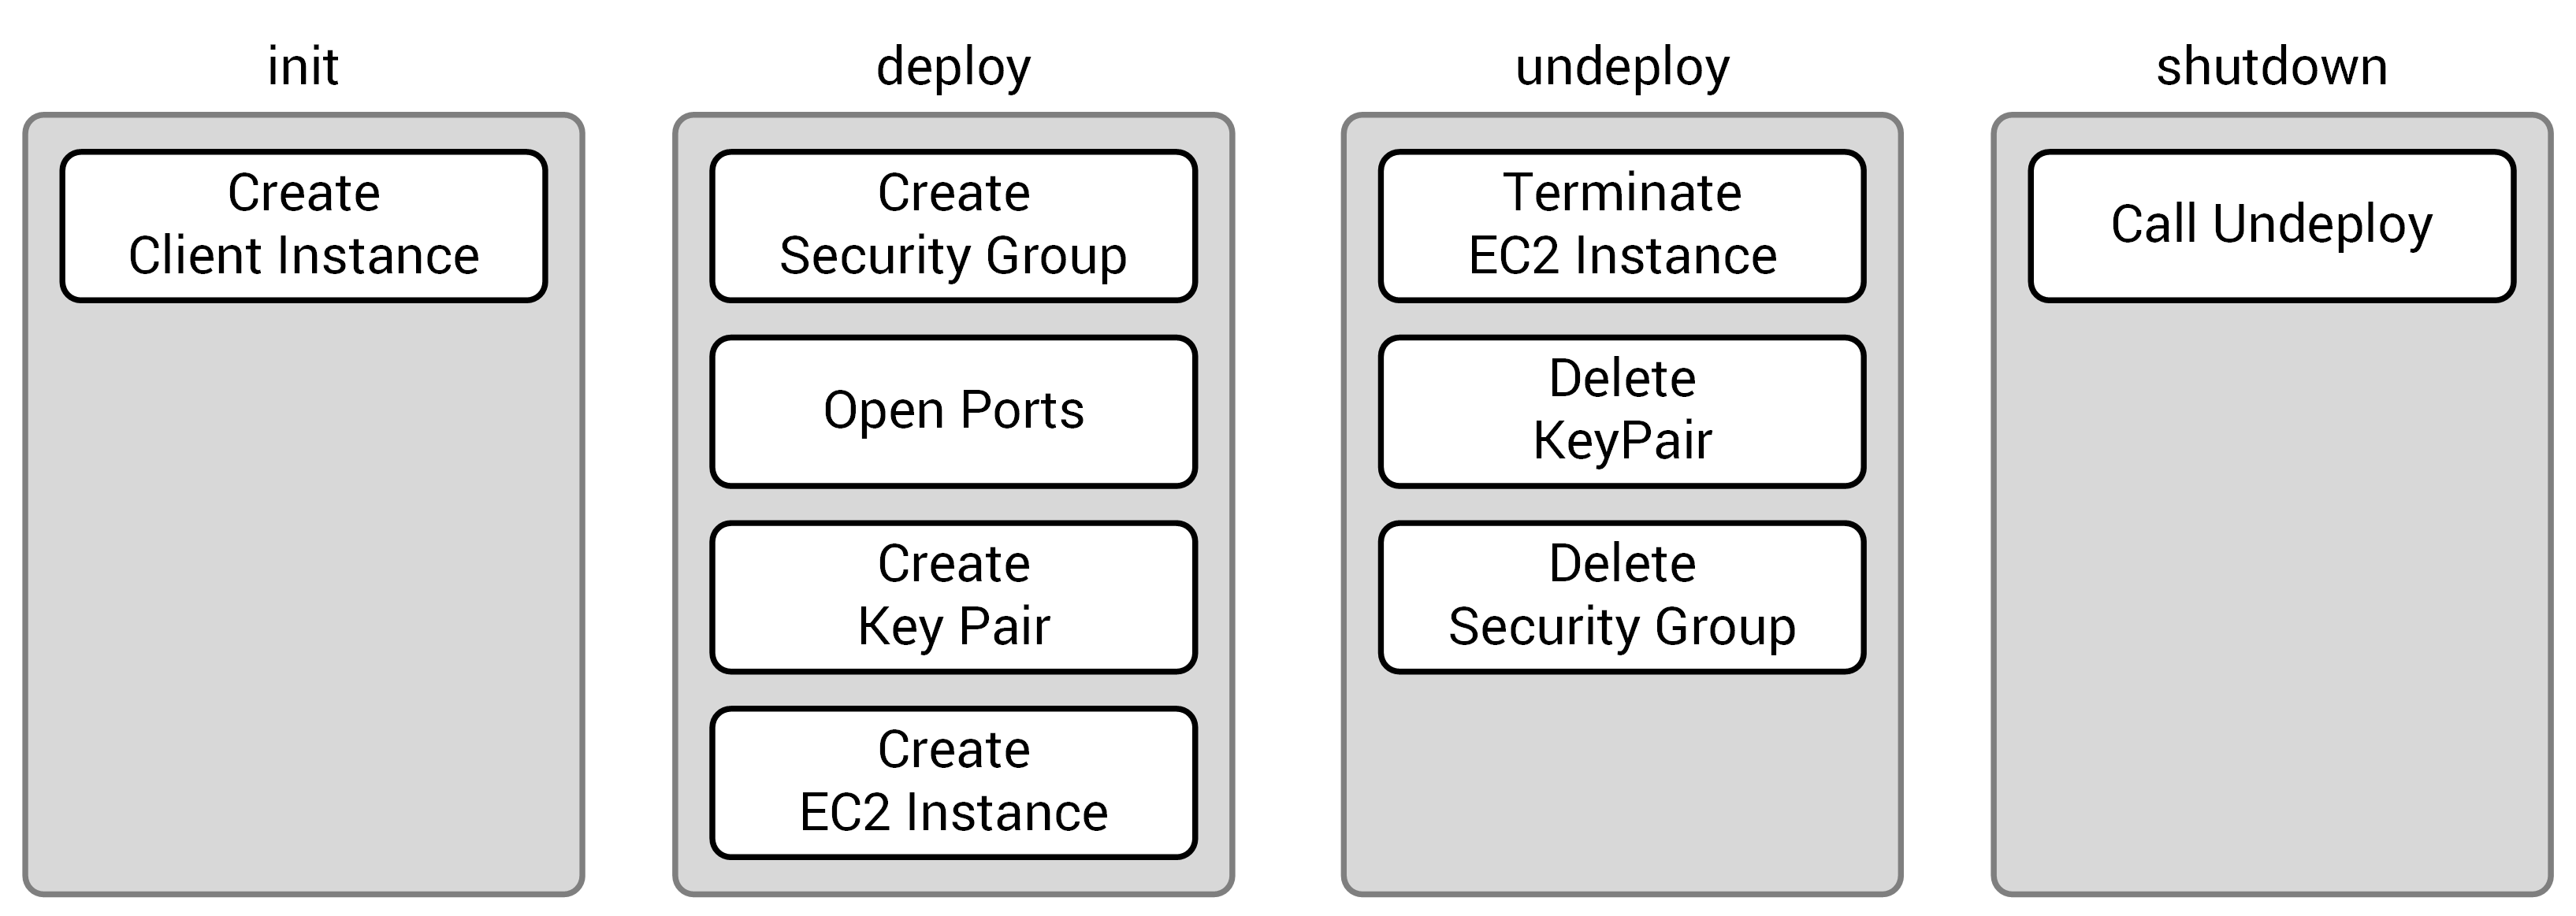
\includegraphics[resolution=600]{implementation/assets/aws_plugin}
	\caption{The operations implemented by the AWS EC2 plugin.}
	\label{image:awsplugin}
\end{figure}

The \textit{initialize} operation, shown on the left of \autoref{image:awsplugin}, which is called once when the plugin is loaded, creates a client instance, which is an object on which all the following actions will be called.
The client instance is bound to a specific AWS region, which is read from the configuration object that is passed into the \textit{initialize} operation.
As we can see in the \textit{deploy} operation in \autoref{image:awsplugin}, we first have to create a security group\footnote{\url{http://docs.aws.amazon.com/AWSEC2/latest/UserGuide/using-network-security.html}}.
Security groups are essentially virtual firewalls that allow or deny traffic to and from all EC2 instances associated with it.
EC2 instances have to be associated with a security group, so we have to create one.
In the next step we open all ports in this security group that we later want to use for communication.
Which ports we open is determined by reading the configuration object.
We also have to create a SSH key pair and retrieve the private key, which we later use when we connect to this EC2 instance via SSH.
In the last step we create the actual EC2 instance.
Once it is up and running, the \textit{deploy} operation is finished and returns an instance object which contains the URL where the EC2 instance can be reached, as well as the private key for SSH access.
The \textit{undeploy} operation reverses the \textit{deploy} operation.
First, it terminates the EC2 instance.
Once the instance is stopped, the key pair and the security group that were created earlier are removed.
We do not have to close the ports we opened, because they are part of the security group and do not exist anymore once the security group is removed.
After this, the EC2 instance created earlier is successfully removed.
There are no further actions necessary during the \textit{shutdown} operation, but for safety we call the \textit{undeploy} operation, in case it was not called earlier.

\subsection{SSH Plugin}

This communication plugin allows the bootware to connect to a remote system via SSH.
It uses the Ganymed SSH-2 library\footnote{\url{https://code.google.com/p/ganymed-ssh-2/}}, which implements the SSH-2 protocol in Java.
\autoref{image:sshplugin} shows a simplified overview of the actions necessary to create a SSH connection and how they map onto the communication plugin operations.

\begin{figure}[!htbp]
	\centering
	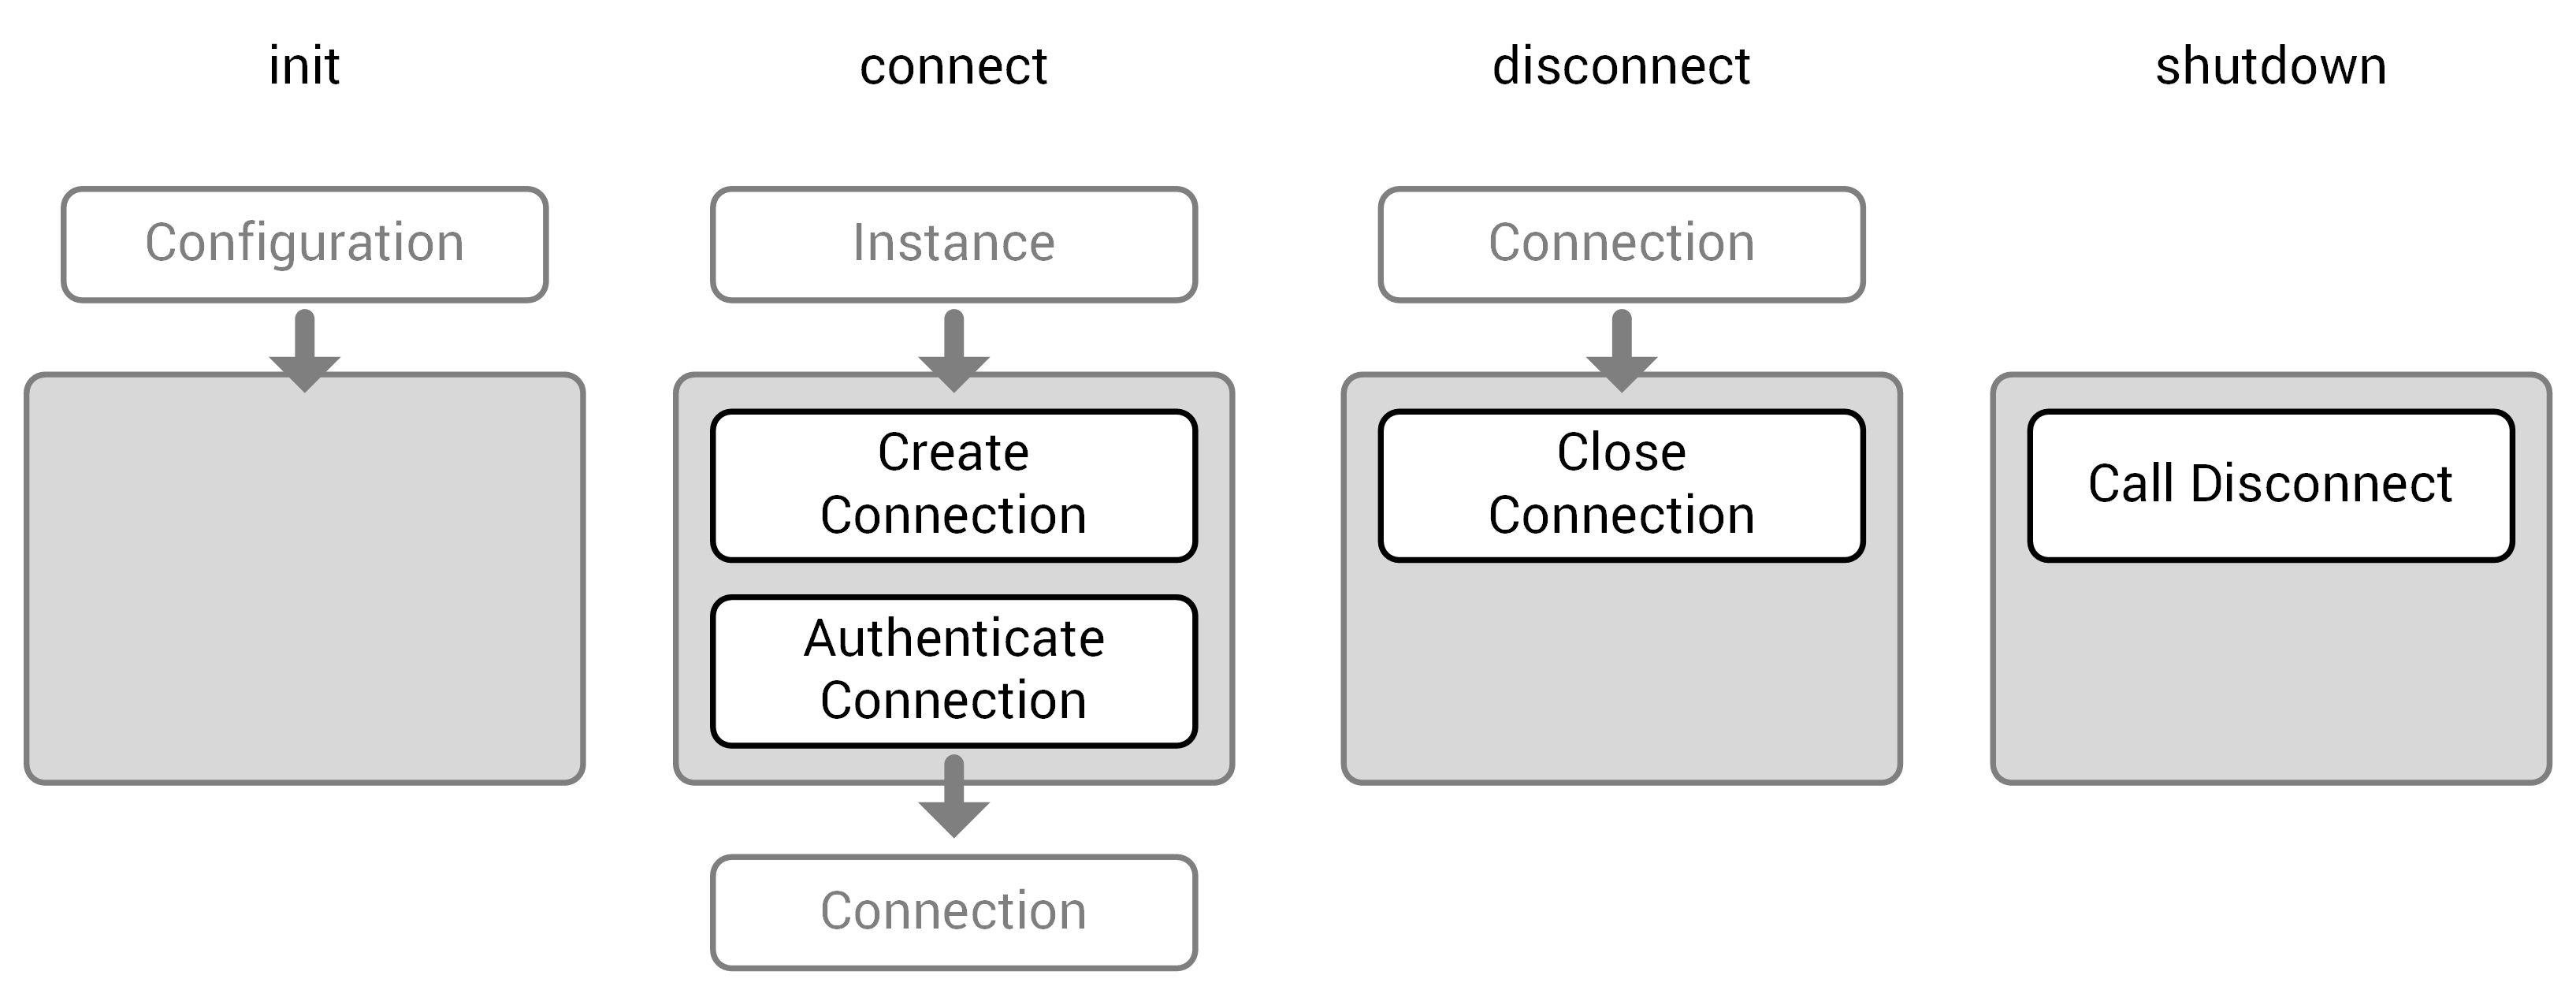
\includegraphics[resolution=600]{implementation/assets/ssh_plugin}
	\caption{The operations implemented by the SSH plugin.}
	\label{image:sshplugin}
\end{figure}

No actions are taken in the \textit{initialize} operation.
During the \textit{connect} operation, we first have to create a connection object, which is bound to a certain host name, i.e. the IP address of the remote system that we want to connect to.
We get this address from the instance object passed into the connect operation.
Then, we have to authenticate this connection.
Multiple authentication methods are supported by SSH-2 protocol, including password and public key authentication.
The necessary values for these authentication methods are read from the instance object passed into the \textit{connect} operation.
Once the connection is authenticated, a connection object is returned, which supports the execute and upload operation that other components can use.

The \textit{disconnect} operation simply closes the connection associated with the connection object that is passed into it.
The \textit{disconnect} operation is also called by the \textit{shutdown} operation at the end of the plugin life cycle to close any connection that might still be open.

\subsection{Remote Bootware Plugin}

This application plugin allows the local bootware to install the remote bootware on a remote system.
\autoref{image:remotebootwareplugin} shows a simplified overview of the steps involved in the installation of the remote bootware and how they map onto the application plugin operations.
The \textit{undeploy} and \textit{stop} operations where omitted because they are not really required in this case.

\begin{figure}[!htbp]
	\centering
	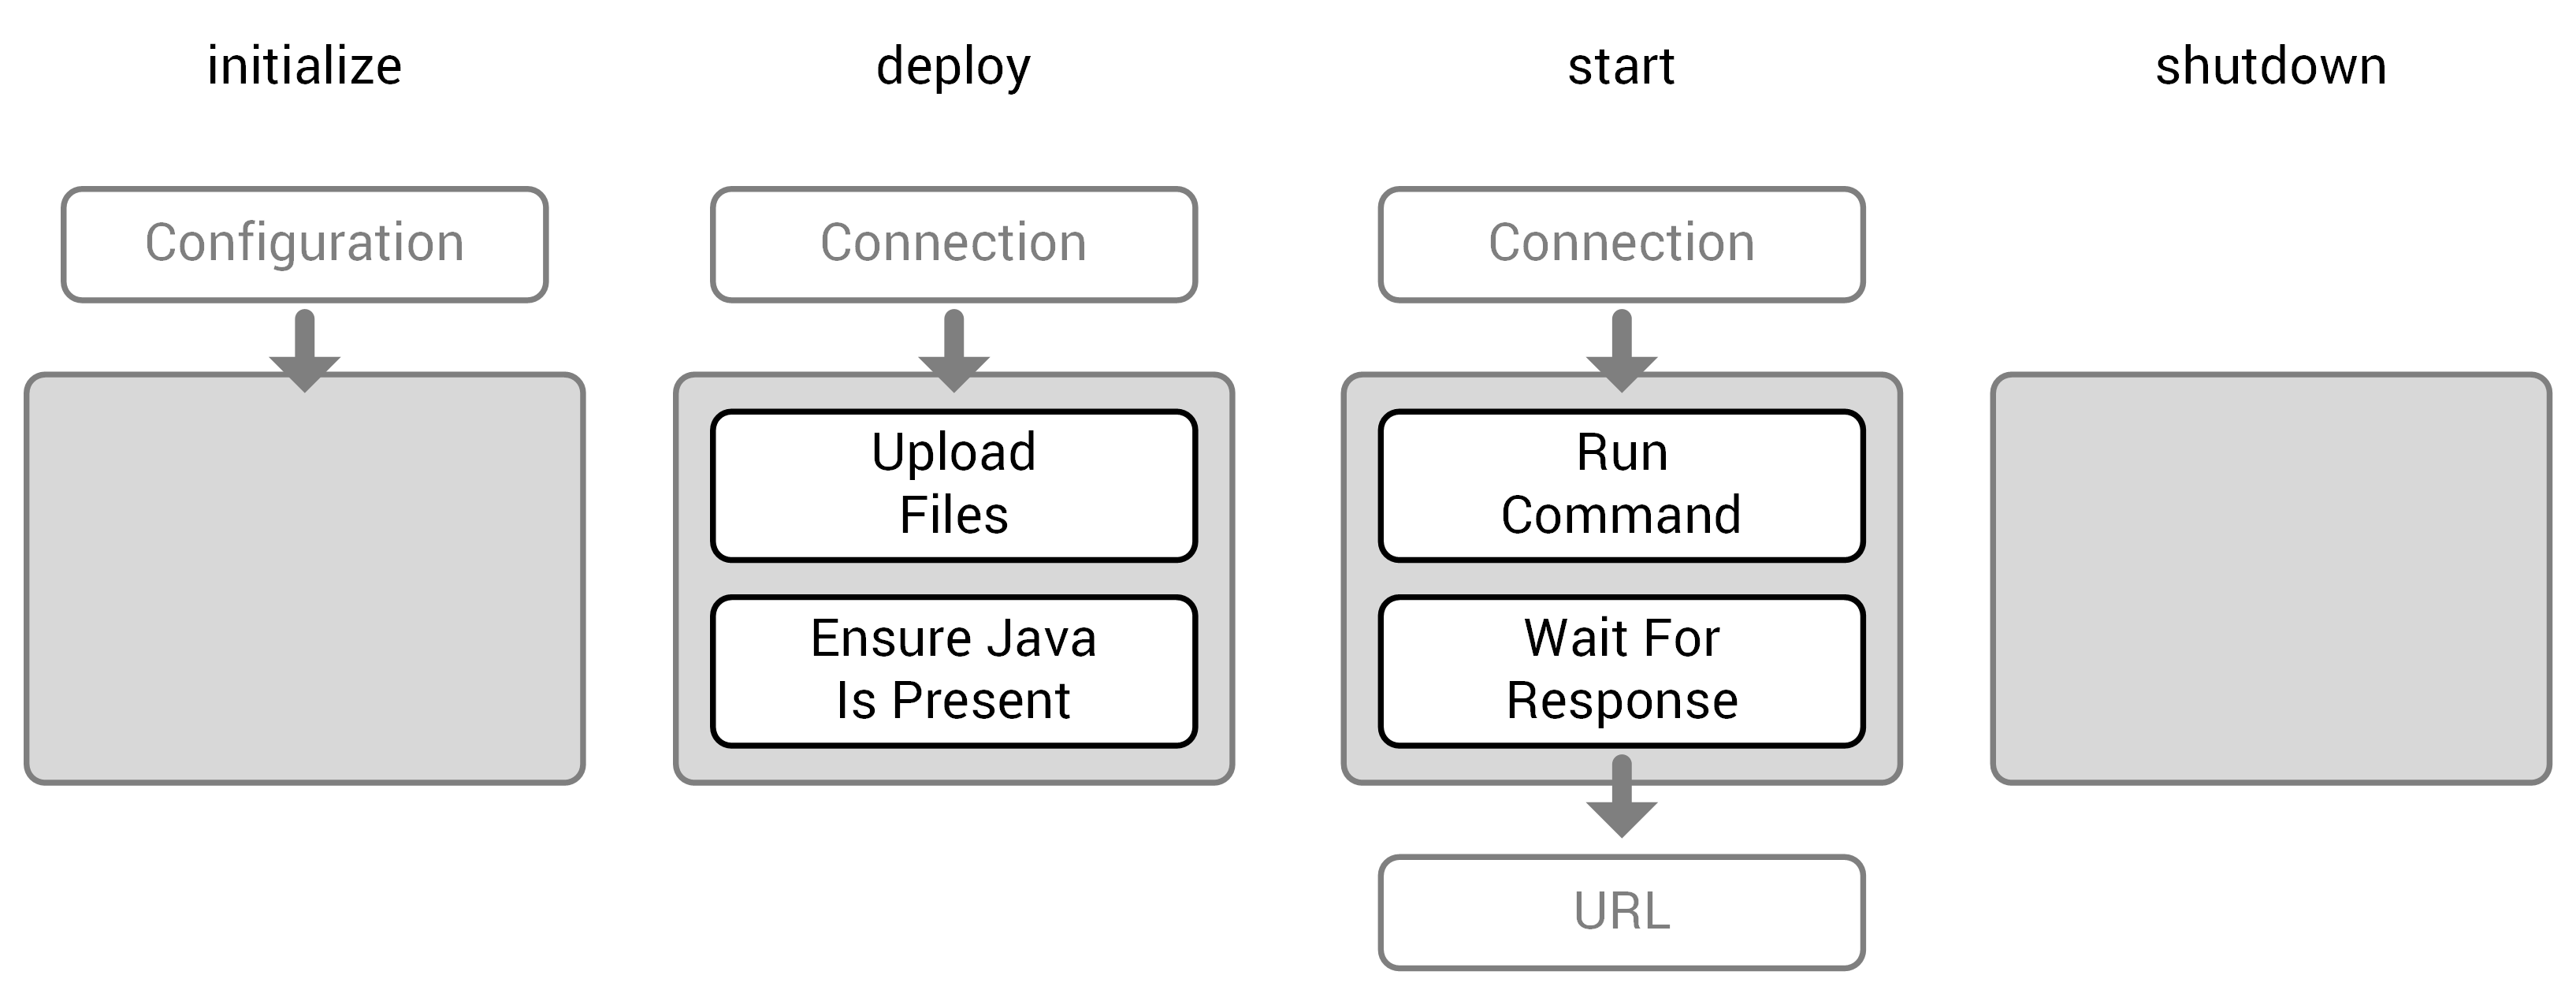
\includegraphics[resolution=600]{implementation/assets/remotebootware_plugin}
	\caption{The operations implemented by the remote bootware plugin.}
	\label{image:remotebootwareplugin}
\end{figure}

In this plugin, the \textit{initialize} operation does not take any actions.
The \textit{deploy} operation first uses the operations provided by the connection object it receives as input to upload the remote bootware files from the local to the remote machine.
Then, it checks if the Java version required to execute the remote bootware is present.
If not, it installs the required Java version.
The remote bootware should now be ready to start.
In the \textit{start} operation a command to execute the remote bootware is sent to the remote machine.
Then, the port for the remote bootware web interface is polled until a response is received, which means that the remote bootware should now be ready.
Finally, the URL to the remote bootware is returned.

\subsection{OpenTOSCA Plugin}

This application plugin allows the bootware to install an OpenTOSCA container on an EC2 instance.
It executes the installation steps described in the OpenTOSCA manual over a connection provided by a communication plugin.
\autoref{image:opentoscaplugin} shows a simplified overview of the steps involved in the installation of OpenTOSCA and how they map onto the application plugin operations.
The \textit{undeploy} and \textit{stop} operations where omitted because they are not really required in this case.

\begin{figure}[!htbp]
	\centering
	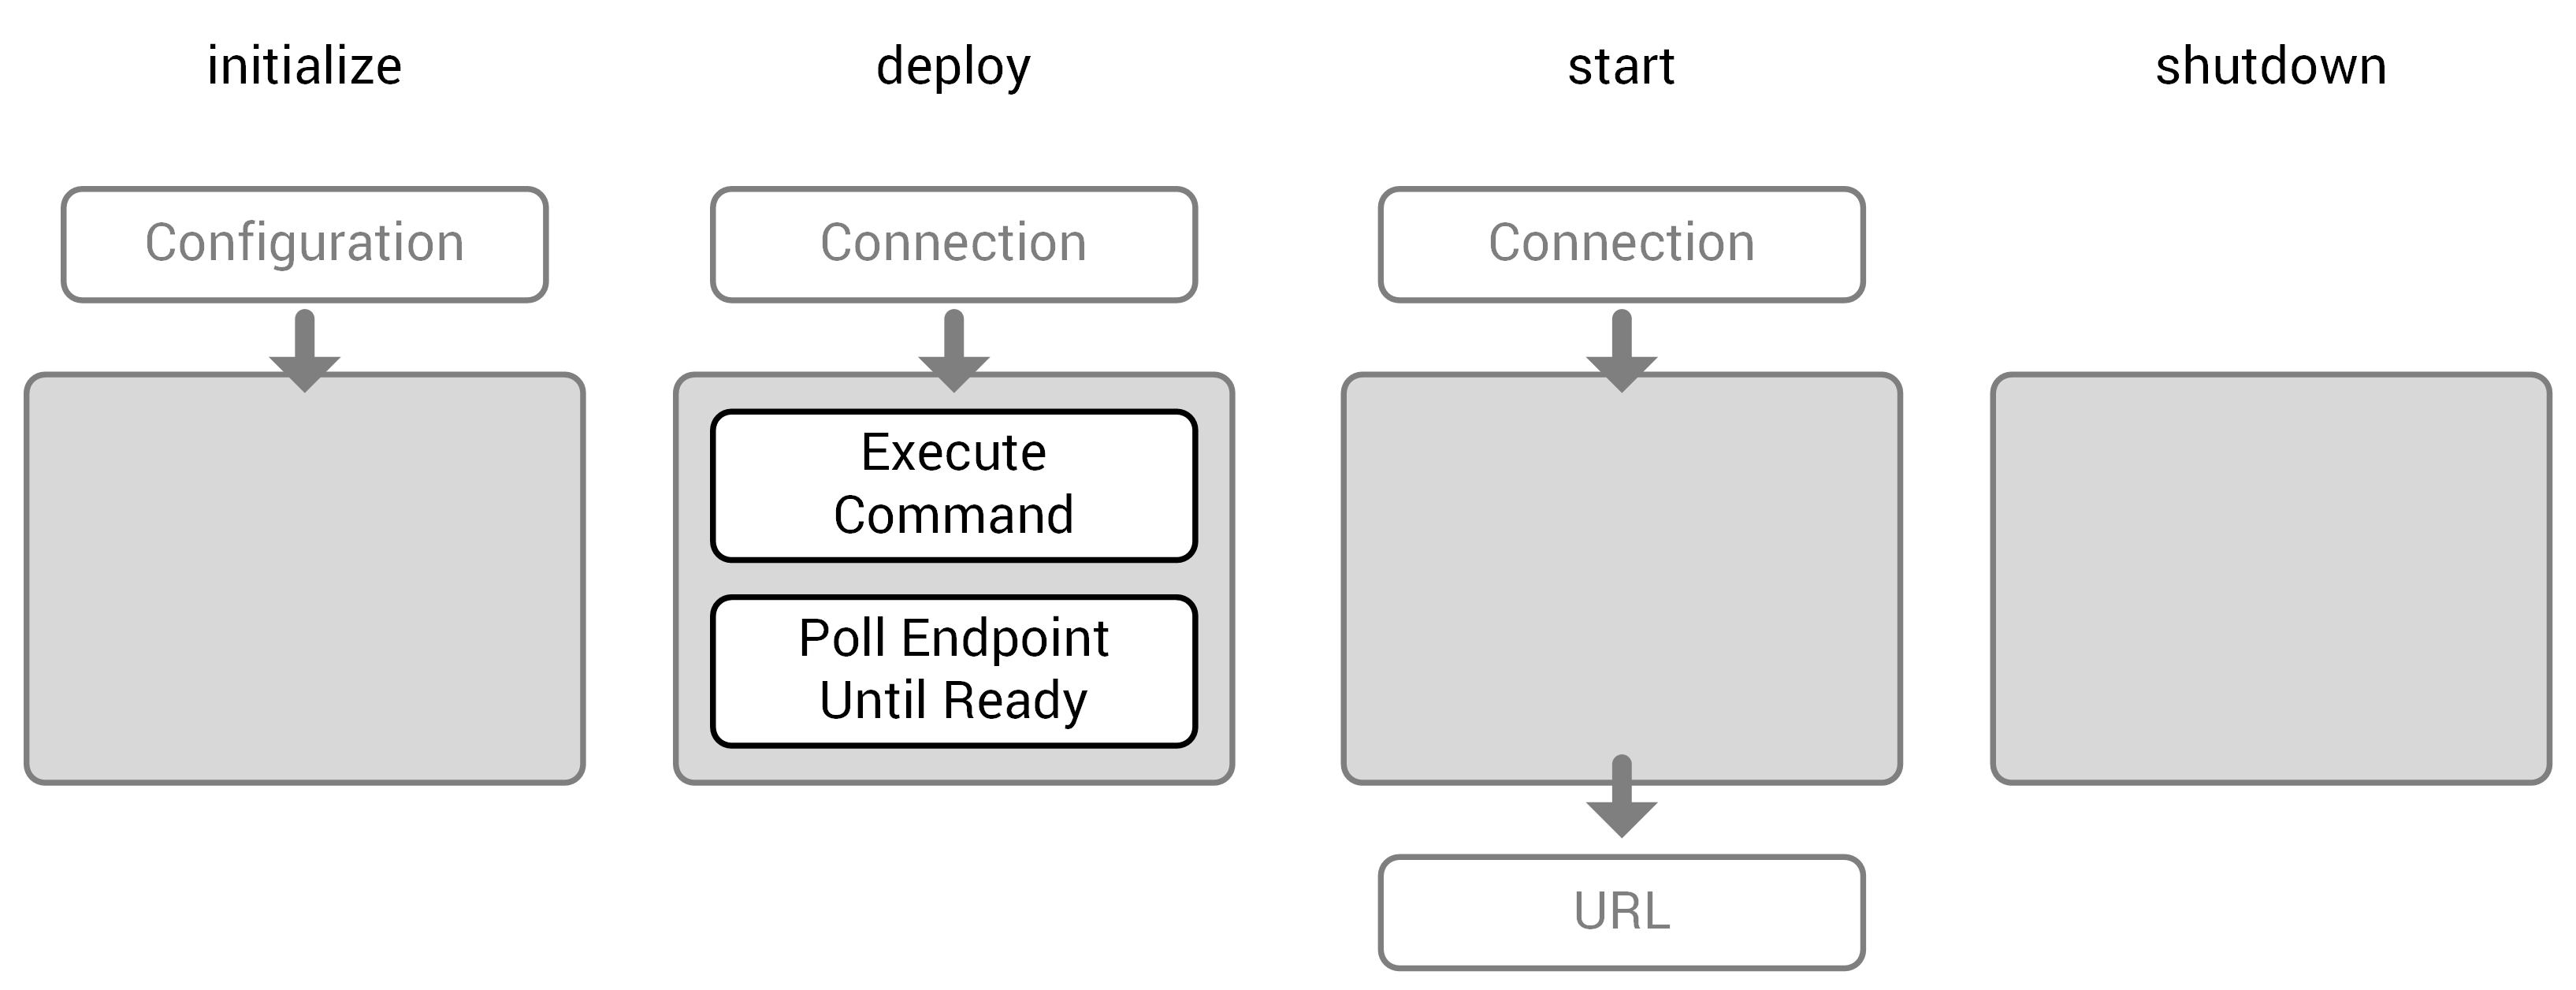
\includegraphics[resolution=600]{implementation/assets/opentosca_plugin}
	\caption{The operations implemented by the OpenTOSCA plugin.}
	\label{image:opentoscaplugin}
\end{figure}

The setup procedure for OpenTOSCA is very simply.
Only one command has to be executed over SSH, which will automatically download and install all necessary components.
After that, port 8080 on the EC2 instance is polled periodically until a connection is possible, which means that the installation process is finished.
The \textit{start} operation only has to return the URL pointing to the OpenTOSCA instance because OpenTOSCA was already started by the installation script.

\subsection{OpenTOSCA Workflow Middleware Plugin}

This provision workflow middleware plugin allows the bootware to provision a workflow middleware using the OpenTOSCA container.
\autoref{image:opentoscamiddlewareplugin} shows a simplified overview of the steps involved in provisioning and deprovisioning the workflow middleware with OpenTOSCA and how they map onto the provision workflow middleware plugin operations.

\begin{figure}[!htbp]
	\centering
	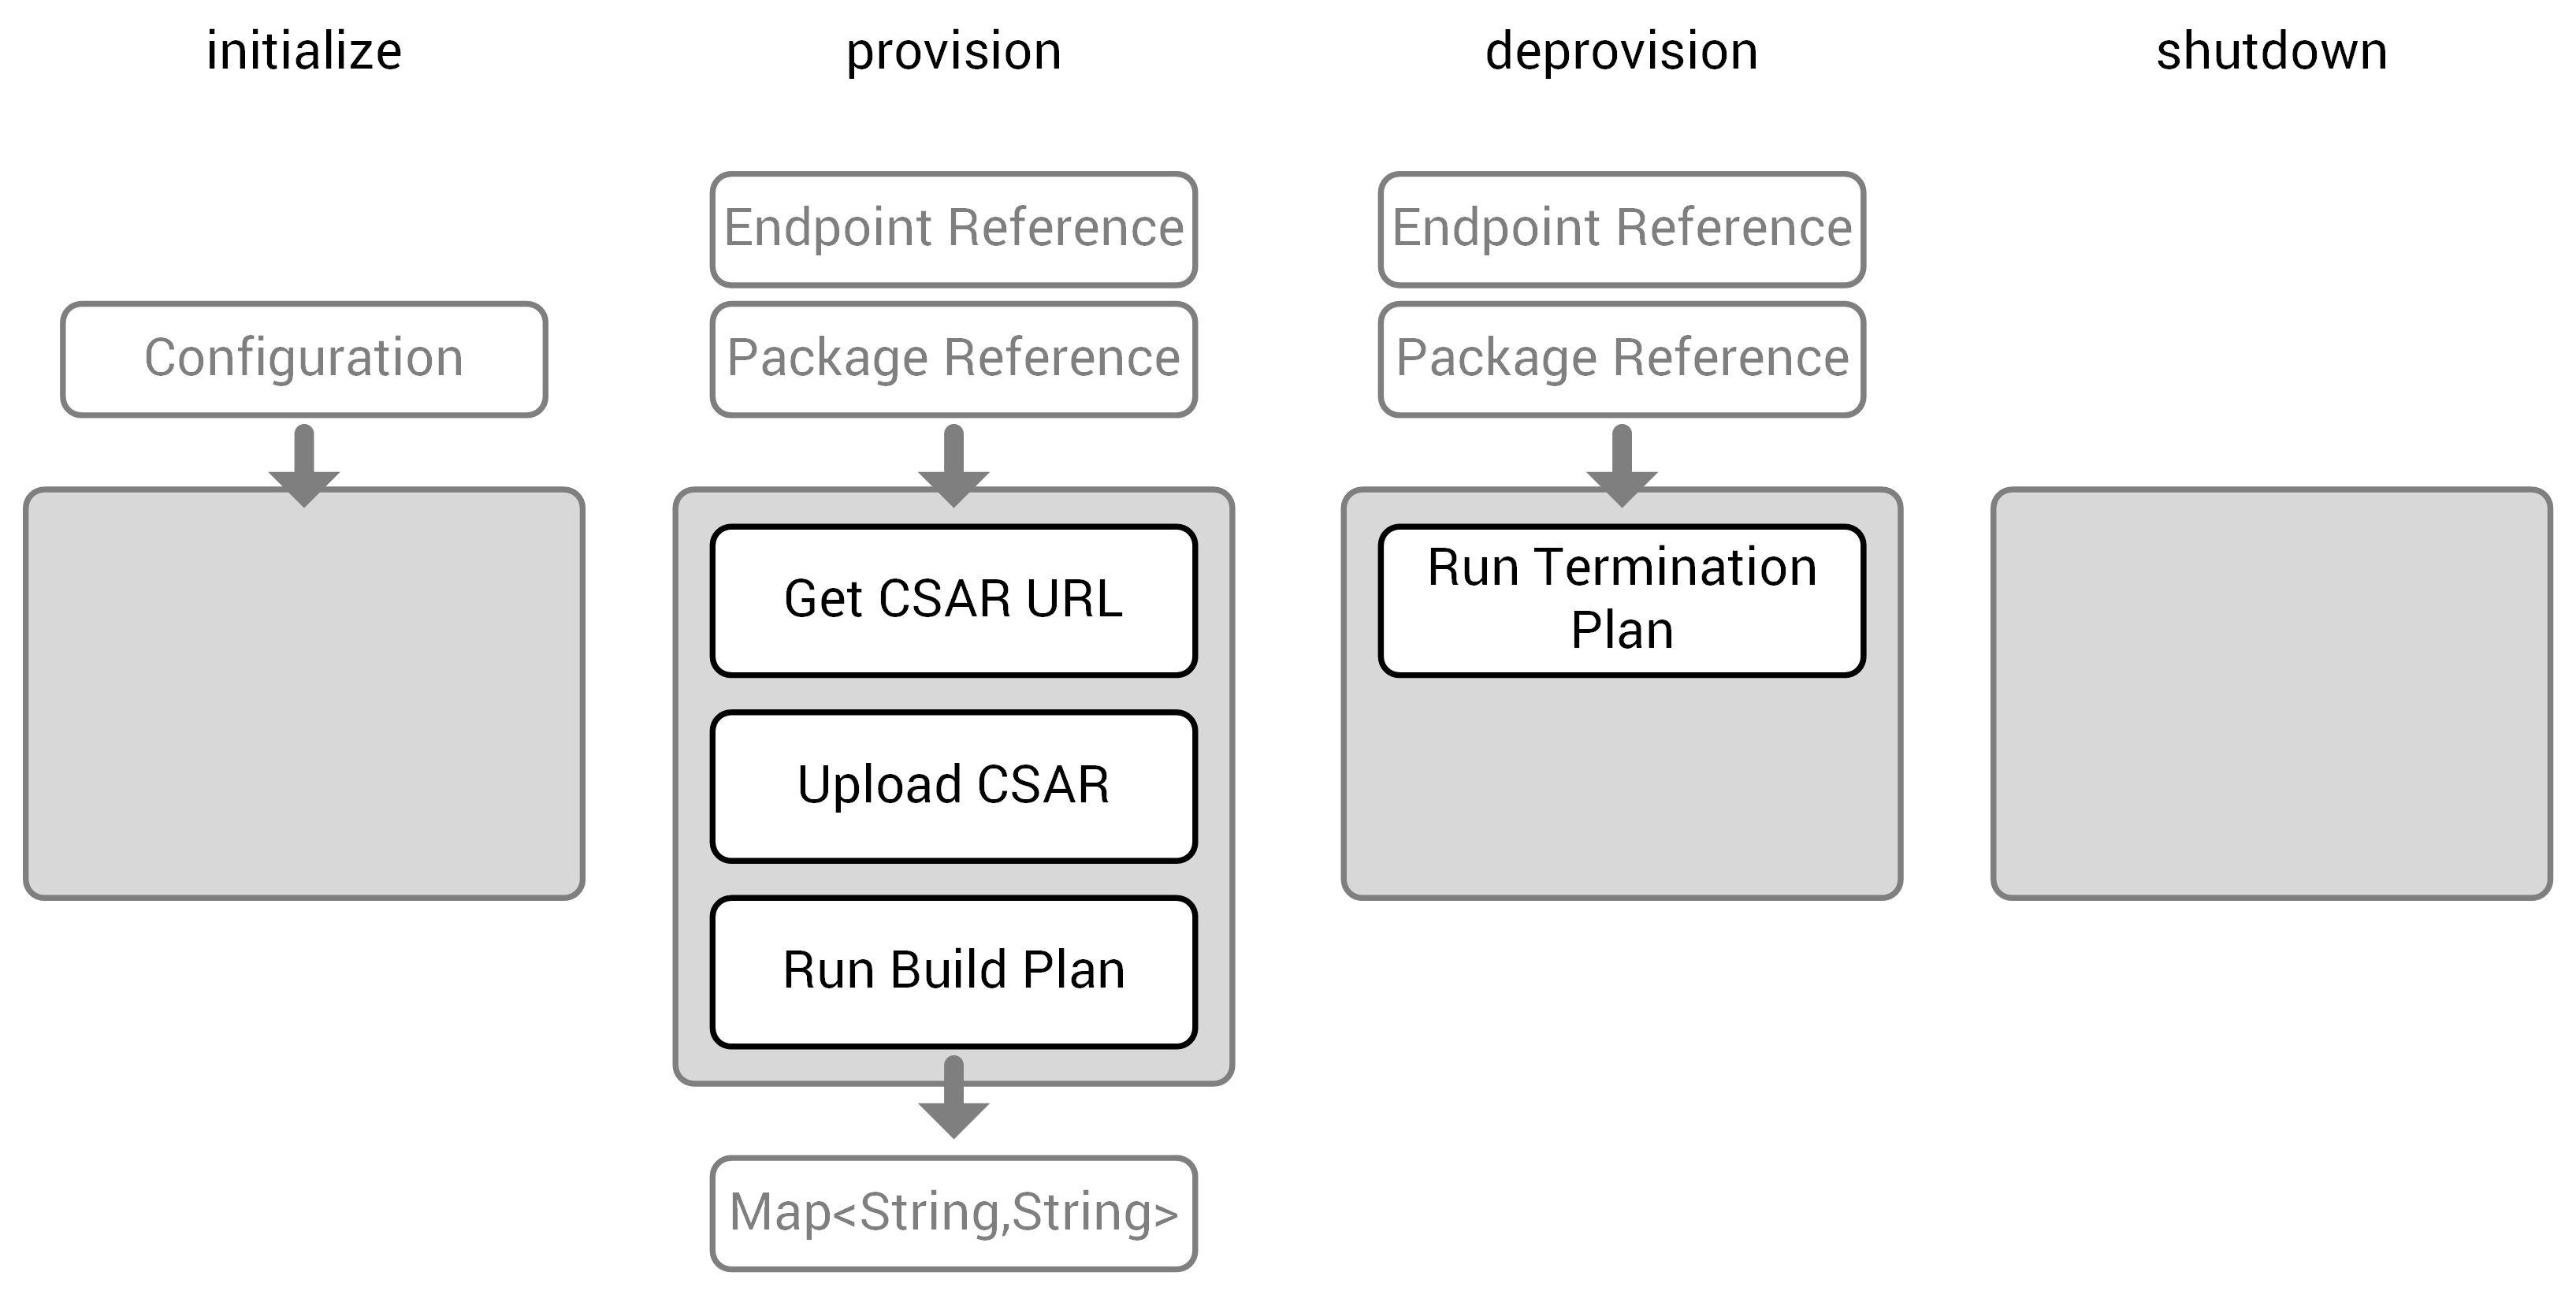
\includegraphics[resolution=600]{implementation/assets/opentosca_middleware_plugin}
	\caption{The operations implemented by the OpenTOSCA workflow middleware plugin.}
	\label{image:opentoscamiddlewareplugin}
\end{figure}

The \textit{initialization} and \textit{shutdown} operations are not used in this plugin.
The \textit{provision} operation first has to get the actual CSAR URL from the service package repository, for which it uses the service package reference that was passed in as parameter.
The CSAR URL is then used to upload the CSAR to the OpenTOSCA container.
Once the CSAR is uploaded, the build plan contained inside it can be executed.
The information it returns after its completion is passed back as Map<String, String> (i.e. the implementation of the information list).
The deprovision operation just executes the termination plan contained in the CSAR.

\subsection{File Logger Plugin}

This event plugin logs all events generated by the bootware to a text file.
\autoref{image:fileloggerplugin} shows a simplified overview of the implementation of this plugin.
The \textit{initialize} operation creates a writer object.
The two event handlers shown in the middle use it to write the events they receive into a text file.
The event handler shown on the left reacts to all events of the type \textit{BaseEvent}, which is the parent event of all events generated by the bootware.
Therefore, it logs any event generated by the bootware into the text file.
The event handler shown on the right reacts to a special \textit{DeadMessage} event type generated by the PubSub library we use, MBassador.
This event is generated each time an event is published to the event bus to which no one subscribed.
Those events are not received by any listener and are therefore dead.
We log them here for debugging purposes.
The \textit{shutdown} operation just closes the write object that was created by the \textit{initialize} operation.

\begin{figure}[!htbp]
	\centering
	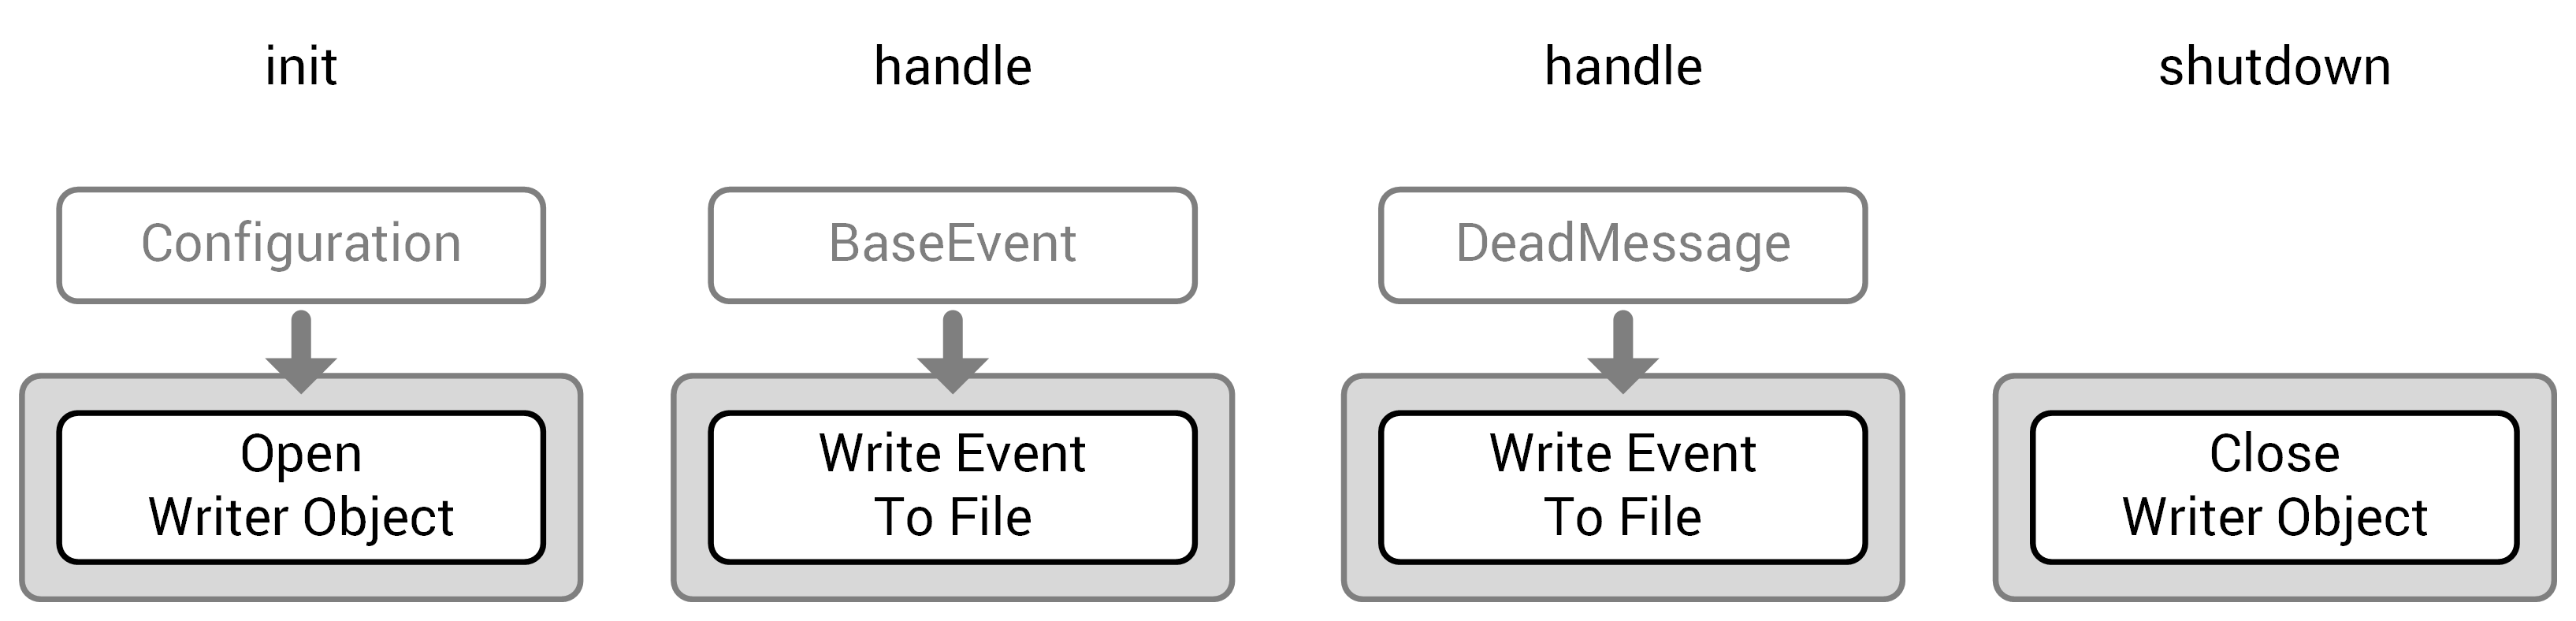
\includegraphics[resolution=600]{implementation/assets/filelogger_plugin}
	\caption{The operations implemented by the file logger plugin.}
	\label{image:fileloggerplugin}
\end{figure}
